\documentclass[a4paper]{article}
\usepackage[italian]{babel}
\usepackage[utf8]{inputenc}
\usepackage{amssymb,amsmath,amsfonts}
\usepackage{graphicx}
\usepackage{listings}

\lstset{basicstyle=\small\tt} 

\author{Guido De Rosa}

\begin{document}

\title{Calcolo numerico del periodo di oscillazione di un pendolo semplice}

\maketitle

\section{Introduzione}

L'energia totale di un pendolo semplice è pari all'energia potenziale
nel punto di massima altezza:
\begin{equation*}
  E = mgh = mg(l - l\cos{\theta_0}) .
\end{equation*}
Per la conservzione dell'energia, nel corso dell'oscillazione è 
\[
  E = mg(l - l\cos{\theta}) + \frac{1}{2}mv^2 . 
\]
Confrontando le ultime due equazioni segue che
\[
  v = \sqrt{2g(\cos{\theta} - \cos{\theta_0})} ,
\] 
ed esprimendo la velocità $v$ come $l\frac{d\theta}{dt}$ si ottiene facilmente:
\[
  dt = \sqrt{\frac{l}{2g}}\frac{d\theta}{\sqrt{\cos{\theta} - \cos{\theta_0} }} .
\]
Integrare in $\theta$ fra $0$ e $\theta_0$ equivale a considerare un quarto di periodo, 
dunque:
\[
  T = 4 \sqrt{\frac{l}{2g}} \int_{0}^{\theta_0}\frac{d\theta}{\sqrt{\cos{\theta}-\cos{\theta_0}}}
\]

Si vuole confrontare questa espressione con l'approssimazione di oscillatore armonico, 
secondo la quale per piccoli valori di $\theta_0$ è:
\[
  T \simeq 2\pi \sqrt{\frac{l}{g}} ,
\]
il che si riconduce, dal punto di vista del calcolo, a verificare la bontà 
dell'approssimazione
\[
  \frac{\pi}{\sqrt{2}} \simeq \int_{0}^{\theta_0}\frac{d\theta}{\sqrt{\cos{\theta}-\cos{\theta_0}}}
\]
per valori sempre più piccoli di $\theta_0$.

\section{Calcolo}
Si sono scelti valori di $\theta_0$ pari a $\frac{\pi}{4}$, $\frac{\pi}{8}$,
$\frac{\pi}{16}$, $\frac{\pi}{32}$, $\frac{\pi}{64}$ e $\frac{\pi}{128}$.  

Per ciascun valore di $\theta_0$, si è suddiviso il dominio di integrazione 
$(0, \theta_0)$ in sottointervalli
di ampiezza $h = \theta_0/2^{n}$, facendo variare $n$ da $8$ a $22$, come si può
vedere da questo estratto del file \texttt{pendulum\_multi.cpp}:
\begin{lstlisting} 
  for (n = (1 << 8); n < (1 << 22); n *= 2) {
    integral.nIntervals = n - 1;
    // exclude the last subinterval, where the f diverges
    integral.upperEnd = theta_0 * ((double)(n - 1)/(double)n);
\end{lstlisting}
dove si vede anche che si è dovuto escludere l'ultimo intervallino, dove 
l'integrando diverge.

I valori dell'integrale $I(h)$ così ottenuti sono poi estrapolati per 
$h\rightarrow0$ (estrapolazione polinomiale):
\begin{lstlisting} 
double integrate(const double theta_0)
{
  PendulumFunction f(theta_0);
  integral::Simpson<PendulumFunction> integral(&f);
  unsigned int n;
  vector< pair<double, double> > extrapolation_points;

  integral.lowerEnd = 0.0;

  for (n = (1 << 8); n < (1 << 22); n *= 2) {
    integral.nIntervals = n - 1;
    // exclude the last subinterval, where the f diverges
    integral.upperEnd = theta_0 * ((double)(n - 1)/(double)n);
    pair<double, double> point(
        integral.deltaX(), integral.compute()
    );
    extrapolation_points.push_back(point);
  }

  interpolator::Polynomial intpl(extrapolation_points);
  return intpl.interpolate(0.0);
}
\end{lstlisting}

Il codice sopra riportato invoca metodi di una libreria appositamente 
realizzata, il cui sorgente è nelle directory 
\texttt{integral/} e \texttt{interpolator/}.

\section{Risultati}
Di seguito è riportato l'output del progamma, i dati ottenuti sono
rappresentati graficamente in Fig. \ref{fig:plot}.
\begin{lstlisting}
# Expected value for small oscillations: 2.22144146908 (PI/sqrt(2))
     0.785398163397       2.3095244447    # theta_0 = PI/4
     0.392699081699      2.24235576036    # theta_0 = PI/8
     0.196349540849      2.22612498591    # theta_0 = PI/16
    0.0981747704247      2.22210097279    # theta_0 = PI/32
    0.0490873852123      2.22109705354    # theta_0 = PI/64
    0.0245436926062      2.22084620366    # theta_0 = PI/128
\end{lstlisting}
\begin{center}
  \begin{figure}

    \begin{center}
      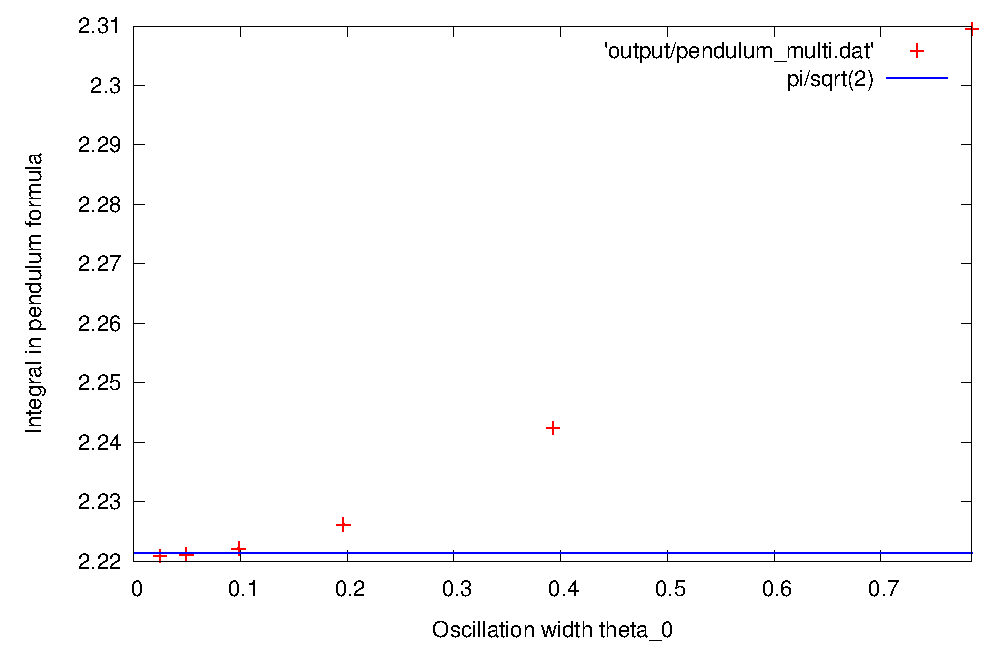
\includegraphics[width=130mm]{plot.pdf}
    \end{center}

    \caption{ Verifica dell'approssimazione $ \frac{\pi}{\sqrt{2}} \simeq \int_{0}^{\theta_0}\frac{d\theta}{\sqrt{\cos{\theta}-\cos{\theta_0}}} $ per $ \theta_0~=~\frac{\pi}{4}, \frac{\pi}{8}, \frac{\pi}{16}, \frac{\pi}{32}, \frac{\pi}{64}, \frac{\pi}{128} $.  }
    
    \label{fig:plot}
    
  \end{figure}
\end{center}

\end{document}
